

\begin{center}
\RRR{25-3}
\end{center}


\begin{tabular}{|c|c|c|c|} \hline 
\multicolumn{4}{|c|}{  \BS{draw}[\RDD{rotate},blue] (0,0)  rectangle  (2,2) ;   }\\ 
\hline  
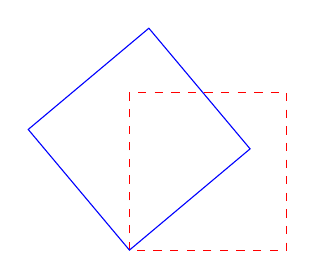
\begin{tikzpicture}
\draw[dashed,red] (0,0) rectangle  (2,2) ; 
\draw[rotate=40,blue] (0,0) rectangle  (2,2) ;
\end{tikzpicture}
&  
\begin{tikzpicture}
\draw[dashed,red] (0,0) rectangle  (2,2) ; 
\draw[x=1cm,y=.5cm,blue] (0,0) rectangle  (2,2); 
\end{tikzpicture}
&  
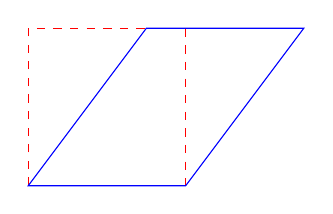
\begin{tikzpicture}
\draw[dashed,red] (0,0) rectangle  (2,2) ; 
\draw[xslant=.75,blue] (0,0) rectangle  (2,2);  
\end{tikzpicture}
&
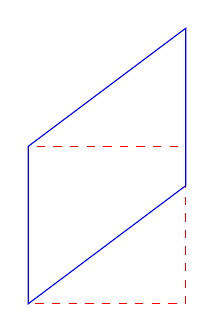
\begin{tikzpicture}
\draw[dashed,red] (0,0) rectangle  (2,2) ; 
\draw[yslant=.75,blue] (0,0) rectangle  (2,2);  
\end{tikzpicture}
\\ \hline  
\RDD{rotate}=40 & \RDD{x}=1cm,\RDD{y}=0.5cm & \RDD{xslant}=0.75 & \RDD{yslant}=0.75\\ 
\hline 
  
\begin{tikzpicture}
\draw[dashed,red] (0,0) rectangle  (2,2) ; 
\draw[scale=1.5,blue] (0,0) rectangle  (2,2) ; 
\end{tikzpicture}
&  
\begin{tikzpicture}
\draw[dashed,red] (0,0) rectangle  (2,2) ; 
\draw[scale=-1,y=.5cm,blue] (0,0) rectangle  (2,2); 
\end{tikzpicture}
&  
\begin{tikzpicture}
\draw[dashed,red] (0,0) rectangle  (2,2) ; 
\draw[xshift=.5cm,blue] (0,0) rectangle  (2,2); 
\end{tikzpicture}
&
\begin{tikzpicture}
\draw[dashed,red] (0,0) rectangle  (2,2) ; 
\draw[yshift=.5cm,blue] (0,0) rectangle  (2,2);  
\end{tikzpicture}
\\ \hline  
\RDD{scale}=1.5 & \RDD{scale}=-1 & \RDD{xshift}=0.5cm & \RDD{yshift}=0.5cm
\\ \hline 
\end{tabular} 

\bigskip
